\documentclass{article}
\usepackage{amssymb}
\usepackage[utf8]{inputenc}
\usepackage{geometry}
\usepackage{mathtools}
\usepackage{verbatim}

\geometry{letterpaper, portrait, margin=1in}

\title{CS325 - Project 1}
\author{Group \#6 \\ William Jernigan, Alexander Merrill, Sean Rettig}
\date{\today}

\begin{document}

\maketitle

\section*{Correctness}
\subsection*{Proof of Claim 2: Direct Proof}

\begin{quote}
Claim 2: If $\{y_{j_1}, y_{j_2},...,y_{j_{t}}\}$ is the visible subset of $\{y_1, y_2,...,y_{i - 1}\} (t \leq i - 1)$ then $\{y_{j_1}, y_{j_2},...,y_{j_{k}}, y_i\}$ is the visible subset of $\{y_1, y_2,...,y_{i}\}$ where $y_{j_{k}}$ is the last line such that $y_{j_{k}} (x^*) \geq y_i (x^*)$ where $(x^*, y_{j_{k}}(x^*))$ is the point of intersection of lines $y_{j_{k}}$ and $y_{j_{k - 1}}$.
\end{quote}

Let $V=\{y_{j_1}, y_{j_2},...,y_{j_{t}}\}$ be the visible subset of $A=\{y_1, y_2,...,y_{i - 1}\}$.

Let $V^+=\{y_{j_1}, y_{j_2},...,y_{j_{k}}, y_i\}$ be the visible subset of $A^+=\{y_1, y_2,...,y_{i}\}$.\\

To prove Claim 2, we must prove that each new line $y_i$ is visible at the time it is added to $V^+$, that each culled line $y_{j_p}$ (where $k < p < i$) was no longer visible due to being covered by $y_i$, and that each remaining line $y_{j_1}$ ... $y_{j_k}$ remains visible in $V^+$.

\subsubsection*{Prove that $y_{i} \in V^+$}
Let $A^+ = A \cup \{y_i\}$.\\
Because $m_i > m_n$ for all $n < i$, $y_i$ is visible by the Claim 1 proof in the "Visible Line Notes" handout.\\
Since $y_i$ is visible and $y_i \in A^+, y_i$ must also be in $V^+$, the visible subset of $A^+$.

\subsubsection*{Prove that $y_{j_k} \in V^+$}
Let $(x^*, y_{j_k} (x^*))$ be the point of intersection of the lines $y_{j_k}$ and $y_{j_{k-1}}$.\\
Since $y_{j_k} (x^*) \geq y_i (x^*)$ by definition, $y_{j_k}$ is visible with respect to $y_i$.\\
Since $y_{j_k}$ was already in $V$, it is defined to be visible with respect to all other elements.\\
$\therefore y_{j_k} \in V^+$.

\subsubsection*{Prove that $y_{j_n} \in V^+, 0 < n < k$}
Because $y_{j_n} \in V$, it is defined to be visible with respect to all other elements in $V$.\\
So we must show that $y_{j_n}$ is visible with respect to $y_i$ as well.\\
Let $(x^*_n, y_{j_n}(x^*_n))$ be the point of intersection of the lines $y_{j_n}$ and $y_{j_{n+1}}$.\\
By definition, $m_{j_n} < m_{j_{n+1}}$, so $\forall x_n < x^*_n, y_{j_n} (x_n) \geq y_{j_{n+1}} (x_n)$.\\
%(x^*_{1,2}) = (x^*_1) by our definition
$\therefore y_{j_{1}}(x^*_{1}) = y_{j_{2}}(x^*_{1}) \geq y_{j_3}(x^*_{1}), y_{j_{2}}(x^*_{2}) = y_{j_{3}}(x^*_{2}) \geq y_{j_4}(x^*_{2}), ..., y_{j_{n-1}}(x^*_{n-1}) = y_{j_{n}}(x^*_{n-1}) \geq y_{j_{n+1}}(x^*_{n-1}), ..., y_{j_{k-1}}(x^*_{k-1}) = y_{j_{k}}(x^*_{k-1}) \geq y_{j_{i}}(x^*_{k-1})$\\
$\therefore y_{j_n}$ is visible with respect to $y_i$.\\
$\therefore y_{j_n} \in V^+$.

\subsubsection*{Prove that $y_{j_p} \notin V^+, k < p < i$}
%Because $y_{j_p} \notin V$, it is defined not to be visible with all other elements.\\
$y_{j_p} \notin V$ if $t < p < i$ or $y_{j_p} \in V$ if $k < p < t$.\\
We must show that $y_{j_p}$ is not visible with respect to $y_i$ as well.

\subsubsection{$y_{j_p} \notin V$ if $t < p < i$}
%I think this is right?
If $y_{j_p}$ was not visible in $V$ then it cannot be visible in $V^+$ by the Claim 1 proof in the "Visible Line Notes" handout.\\

\subsubsection{$y_{j_p} \in V$ if $k < p \leq t$}

\begin{comment}
This is what I've been fiddling with for the proof this morning.

%used p & p-1 so that it goes from intersects of k to t, p+1 would go from k+1 to t+1.
Let $(x^*_p, y_{j_p}(x^*_p))$ be the point of intersection of the lines $y_{j_{p-1}}$ and $y_{j_{p}}$.\\
By definition, $m_{j_{p-1}} < m_{j_{p}}$, so $\forall x_{p-1} < x^*_{p-1}, y_{j_{p-1}} (x_{p-1}) \geq y_{j_{p}} (x_{p-1})$.\\
Since $y_{j_p}$ was already in $V$, it is defined to be visible with respect to all other elements.\\
$\therefore y_{j_{1}}(x^*_{2}) = y_{j_{2}}(x^*_{2}) \geq y_{j_3}(x^*_{2}), y_{j_{2}}(x^*_{3}) = y_{j_{3}}(x^*_{3}) \geq y_{j_4}(x^*_{3}), ..., y_{j_{k-1}}(x^*_{k}) = y_{j_{k}}(x^*_{k}) \geq y_{j_{k+1}}(x^*_{k}), ..., y_{j_{p-1}}(x^*_{p}) = y_{j_{p}}(x^*_{p}) \geq y_{j_{p+1}}(x^*_{p}), ..., y_{j_{t-2}}(x^*_{t-1}) = y_{j_{t-1}}(x^*_{t-1}) \geq y_{j_{t}}(x^*_{t-1})$\\
In order for $y_{j_p}$ to not be visible in $V^+$, $y_i (x^*_p) > y_p (x^*_p)$ by definition of visible.\\
%(x^*_{1,2}) = (x^*_2) by our definition
$\therefore y_{j_{1}}(x^*_{2}) = y_{j_{2}}(x^*_{2}) \geq y_{j_3}(x^*_{2}), y_{j_{2}}(x^*_{3}) = y_{j_{3}}(x^*_{3}) \geq y_{j_4}(x^*_{3}), ..., y_{j_{k-1}}(x^*_{k}) = y_{j_{k}}(x^*_{k}) \geq y_{j_{i}}(x^*_{k}), ..., y_{j_{p-1}}(x^*_{p-1,p}) = y_{j_{p}}(x^*_{p-1,p}) < y_{j_{i}}(x^*_{p-1,p}), ..., y_{j_{t-1}}(x^*_{t}) = y_{j_{t}}(x^*_{t}) < y_{j_{i}}(x^*_{t})$\\
Since $y_{j_p}$ was already in $V$, it is defined to be visible with respect to all other elements.\\
$\therefore y_{j_p} \notin V^+$.
\end{comment}

%used p & p-1 so that it goes from intersects of k to t, p+1 would go from k+1 to t+1.
Let $(x^*_p, y_{j_p}(x^*_p))$ be the point of intersection of the lines $y_{j_{p-1}}$ and $y_{j_{p}}$.\\
By definition, $m_{j_{p-1}} < m_{j_{p}}$, so $\forall x_{p-1} < x^*_{p-1}, y_{j_{p-1}} (x_{p-1}) > y_{j_{p}} (x_{p-1})$.\\
$\therefore y_{j_{1}}(x^*_{1,2}) = y_{j_{2}}(x^*_{1,2}) \geq y_{j_3}(x^*_{1,2}), y_{j_{2}}(x^*_{2,3}) = y_{j_{3}}(x^*_{2,3}) \geq y_{j_4}(x^*_{2,3}), ..., y_{j_{p-1}}(x^*_{p-1,p}) = y_{j_{p}}(x^*_{p-1,p}) \geq y_{j_{p+1}}(x^*_{p-1,p}), ..., y_{j_{k-1}}(x^*_{k-1,k}) = y_{j_{k}}(x^*_{k-1,k}) \geq y_{j_{i}}(x^*_{k-1,k})$\\
Since $y_{j_p}$ was already in $V$, it is defined to be visible with respect to all other elements.\\
$\therefore y_{j_p} \in V^+$.

\subsection*{Proof of Algorithm 3: Direct Proof}
As Algorithm 3 is simply an implementation of Claim 2, and Claim 2 was proven above, Algorithm 3 is also proven to be correct.  Our Claim 2 proof shows that each new line $y_i$ is visible at the time it is added to $V^+$, that each culled line $y_{j_p}$ was no longer visible due to being covered by $y_i$, and that each remaining line $y_{j_1}$ ... $y_{j_k}$ remains visible in $V^+$.

\section*{Experimental and Asymptotic Run Time Analysis}
\subsection*{Experimental Run Time Data}
\verbatiminput{times.txt}

\pagebreak

\subsection*{Experimental Run Time Plots}
\centerline{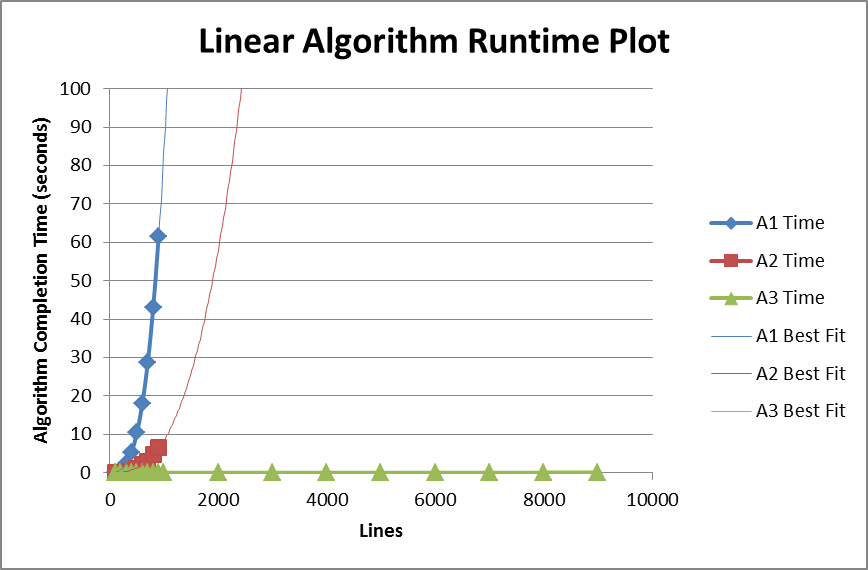
\includegraphics[width=0.75\textwidth]{plot1.png}}
\centerline{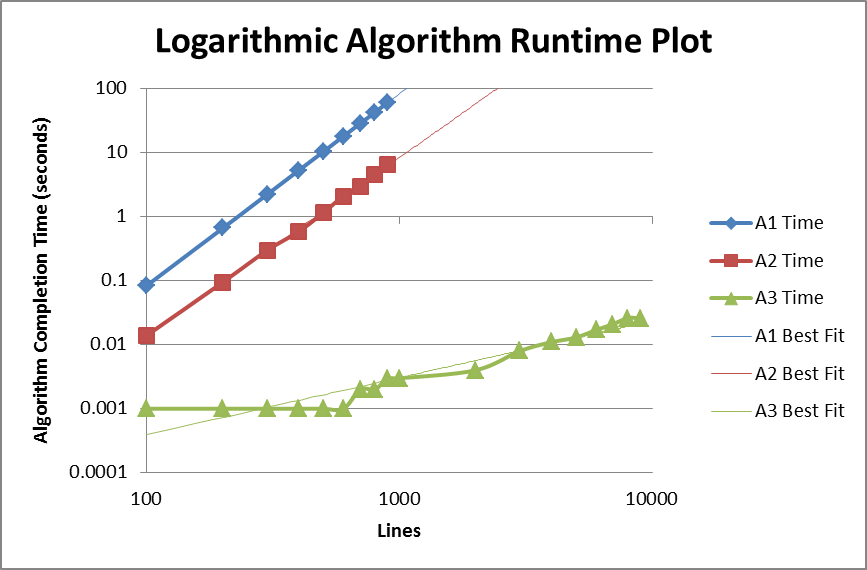
\includegraphics[width=0.75\textwidth]{plot2.png}}

\pagebreak

\subsection*{Experimental Run Time Analysis}
Algorithm 1: $y=8 \times 10^{-8}x^{3.0026}$\\
Algorithm 2: $y=4 \times 10^{-8}x^{2.7892}$\\
Algorithm 3: $y=7 \times 10^{-6}x^{0.8868}$\\

Given these equations, we can use both the slopes and our code to analyze the run times of the algorithms.

\subsection*{Asymptotic Run Time Analysis}
Algorithm 1: $\Theta(n^3)$\\
\indent Algorithm 1 iterates over the set of lines in a triple-nested loop.\\\\
Algorithm 2: $\Theta(n^3)$\\
\indent Similar to Algorithm 1, Algorithm 2 still has the triple-nested loop---it simply bypasses some unnecessary calculations within the triple-nested loop to speed it up.\\\\
Algorithm 3: $\Theta(n)$\\
\indent Algorithm 3 only iterates over the set of lines once.  Though the removeCovered function can recurse several times, it does not scale with the size of the input list.

\subsection*{Discrepancies}
We note that the slopes from our experimentally-derived equations are close to $\Theta(n^3)$, $\Theta(n^3)$, and $\Theta(n)$, but not exact.  These discrepancies have many possible contributing factors, including a small sample size, a low timing resolution (particularly for Algorithm 3), and randomness in run time present in Algorithms 2 and 3 (which unlike Algorithm 1, do not simply perform a fixed number of operations, but rather change what operations they run depending on the input lines given.  This randomness is likely to be the primary cause, as the experimental running time for Algorithm 1 is by far the closest to our asymptotic estimation.

\subsection*{Estimated Number of Lines Per Hour}
Algorithm 1: $\sim 3,532$\\
Algorithm 2: $\sim 8,460$\\
Algorithm 3: $\sim 7,919,210,000$

\pagebreak

\section*{Pseudocode}
\verbatiminput{pseudocode.txt}

\end{document}
